% Main-text figures. Three-seed error bars show sample SD, not confidence intervals.
\begin{figure*}[t]
\centering
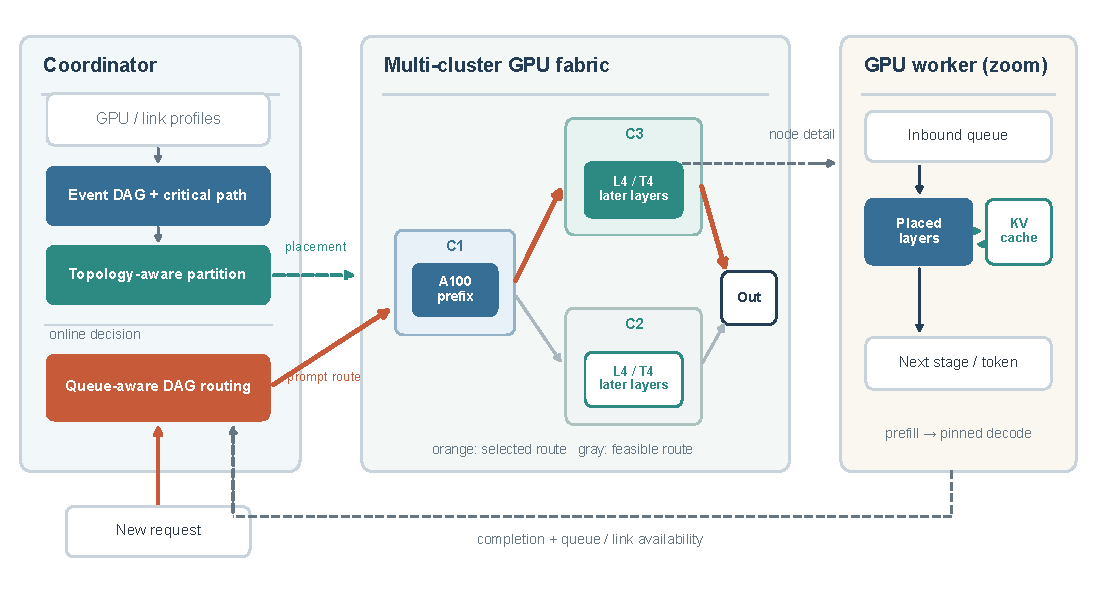
\includegraphics[width=0.95\textwidth]{experiments/paper_figures/ccf_integrated_framework.pdf}
\caption{Integrated overview of the proposed serving system (schematic). The coordinator uses GPU and link profiles to construct a resource-dependent event DAG, identifies critical resources, and produces a capacity- and topology-aware model placement. At prompt admission, a queue-aware layered-DAG search selects a feasible GPU route. The multi-cluster fabric executes the placed layers; each worker manages its inbound queue, model layers, and KV cache. Completion and resource availability feed the next scheduling decision, while decode iterations retain the selected route for KV locality. Colored arrows mark one selected route; gray arrows mark another feasible route. Exact layer intervals are reported separately.}
\label{fig:method-overview}
\end{figure*}

\begin{figure*}[t]
\centering
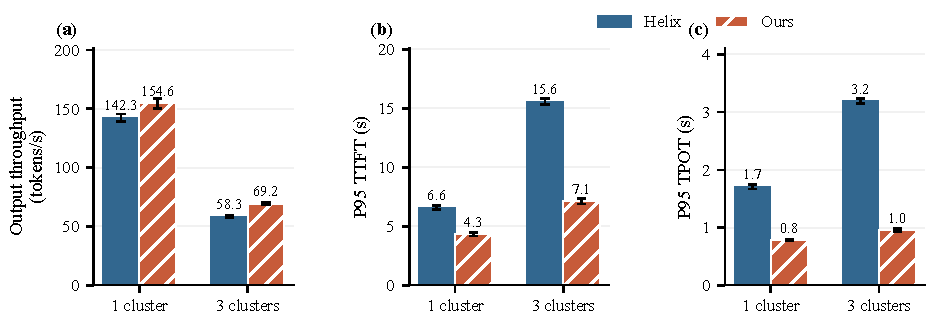
\includegraphics[width=0.95\textwidth]{experiments/paper_figures/fig01_main_performance.pdf}
\caption{End-to-end online serving at the Helix artifact's offered loads. (a) Output-token throughput; (b) 95th-percentile time to first token (TTFT); (c) 95th-percentile time per output token (TPOT). Single-cluster and three-cluster offered loads are 700 and 320 tokens/s, respectively. Bars show means across seeds 0--2; error bars show sample standard deviations, not confidence intervals. Each baseline--candidate pair uses the same trace, zero warmup, and an 1800 s fixed window.}
\label{fig:main-performance}
\end{figure*}

\begin{figure*}[t]
\centering
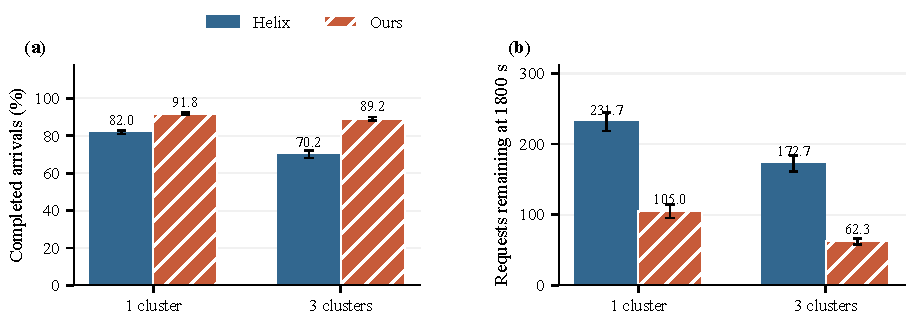
\includegraphics[width=0.95\textwidth]{experiments/paper_figures/fig02_completion_backlog.pdf}
\caption{Request completion and fixed-window censoring for the same three-seed official-load runs as Fig.~\ref{fig:main-performance}. (a) Fraction of arrivals completed by 1800 s; (b) requests still present at 1800 s. Bars show means and sample standard deviations. Unfinished requests are not drained after the measurement window.}
\label{fig:completion-backlog}
\end{figure*}

\begin{figure*}[t]
\centering
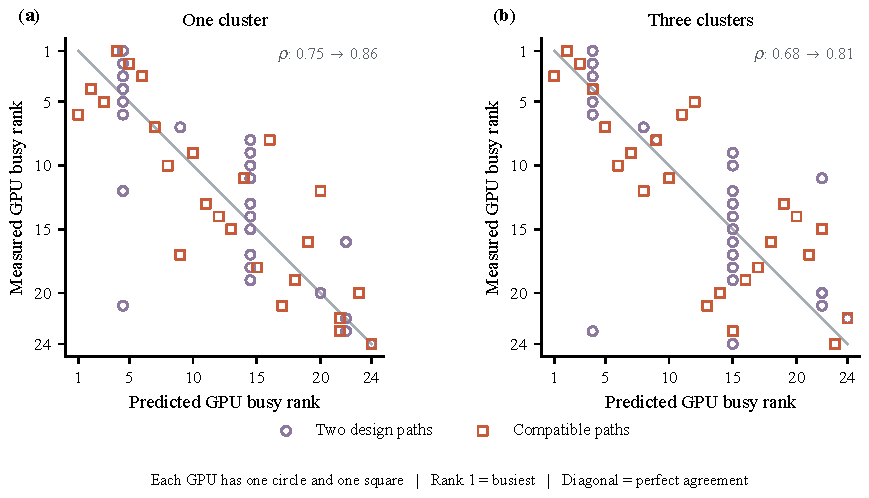
\includegraphics[width=0.95\textwidth]{experiments/paper_figures/fig03_bottleneck_ranks.pdf}
\caption{Agreement between analytic GPU-demand rank and simulated GPU-busy rank in (a) one cluster and (b) three clusters. Rank 1 denotes the busiest GPU; the diagonal is perfect agreement. Spearman's $\rho$ improves from 0.75 to 0.86 and from 0.68 to 0.81 when moving from demand on the two designed branches to demand over all layer-compatible paths. Each panel contains 24 GPUs from one seed-1, 240 s resource profile after 60 s warmup. The audit placement differs from the final official-load placement.}
\label{fig:bottleneck-ranks}
\end{figure*}

\begin{figure*}[t]
\centering
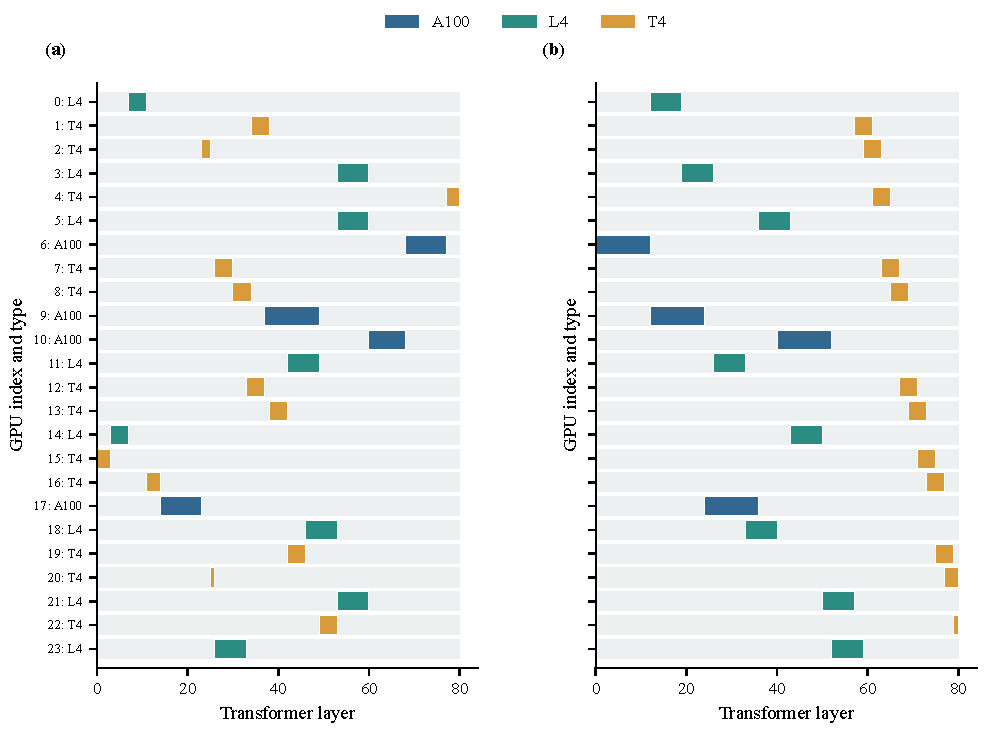
\includegraphics[width=0.95\textwidth]{experiments/paper_figures/fig04_single_placement.pdf}
\caption{GPU-layer assignment for 80 transformer layers in the single-cluster configuration: (a) the official Helix placement and (b) the final graph-partition placement. Colored intervals show the layers loaded on each GPU; colors identify GPU type. Layer and GPU indices are zero-based.}
\label{fig:single-placement}
\end{figure*}

\begin{figure*}[t]
\centering
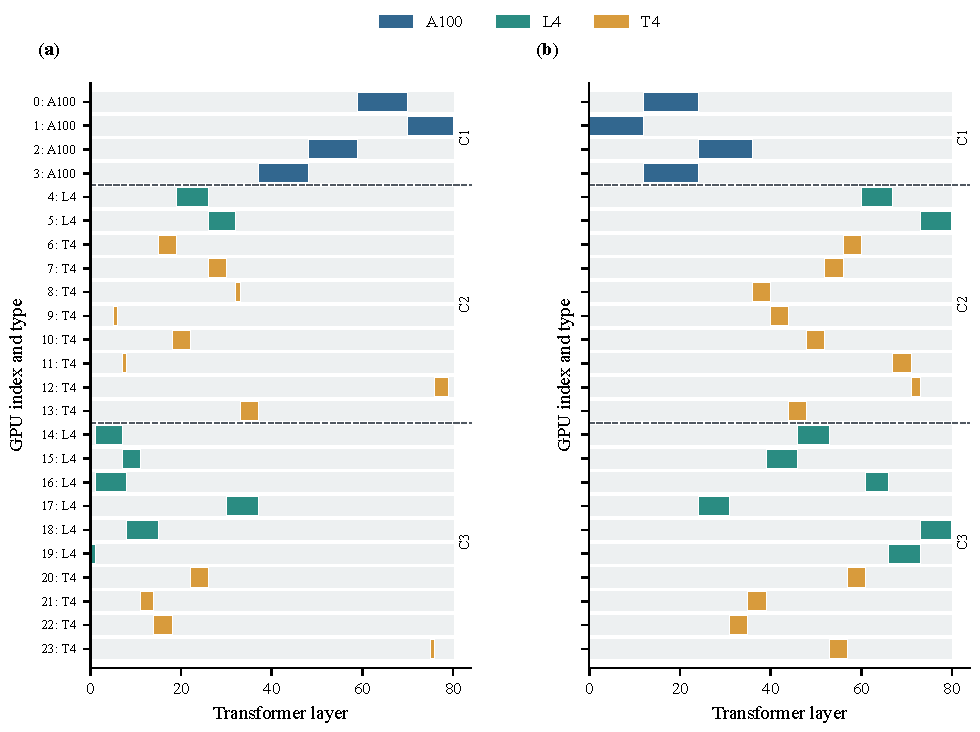
\includegraphics[width=0.95\textwidth]{experiments/paper_figures/fig05_multi_placement.pdf}
\caption{GPU-layer assignment in the three-cluster configuration: (a) the official Helix placement and (b) the final graph-partition placement. Dashed horizontal lines separate physical clusters C1, C2, and C3; colors identify GPU type. The placement is capacity-constrained and contains a shared prefix plus two full suffix paths. Layer and GPU indices are zero-based.}
\label{fig:multi-placement}
\end{figure*}

\begin{figure*}[t]
\centering
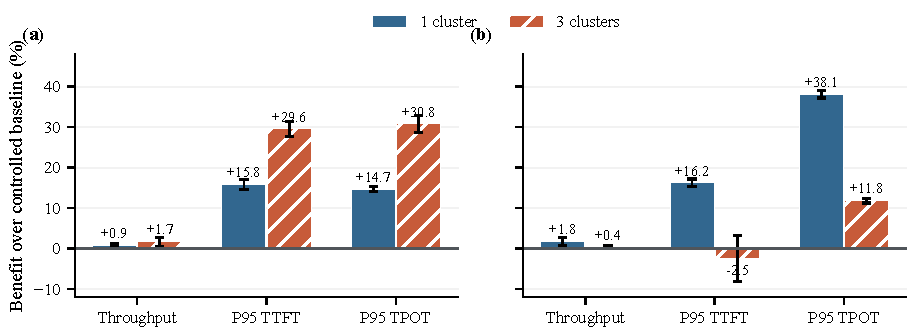
\includegraphics[width=0.95\textwidth]{experiments/paper_figures/fig06_component_attribution.pdf}
\caption{Controlled component comparisons at development offered loads (400 and 160 tokens/s for one and three clusters). Positive values indicate a throughput increase or a P95 latency reduction. (a) Replace only model placement while holding the early layer-DAG scheduler fixed. (b) Replace only scheduling while holding the final placement fixed. Bars show the mean paired benefit across seeds 0--2; error bars show sample standard deviations. Each run has 180 s warmup and 1800 s measurement. These are distinct paired controls; their percentages are not additive.}
\label{fig:component-attribution}
\end{figure*}

\begin{figure}[t]
\centering
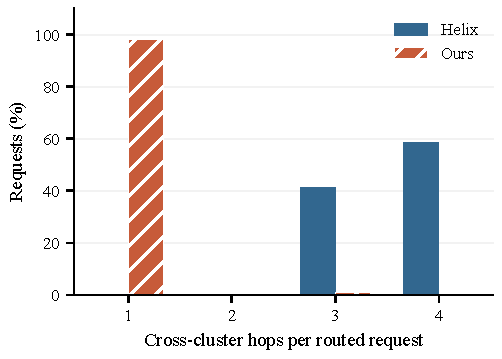
\includegraphics[width=0.48\textwidth]{experiments/paper_figures/fig08_cross_cluster_hops.pdf}
\caption{Number of physical-cluster transitions along each routed request path in the three-cluster official-load run. A transition is counted when consecutive compute stages reside in different partitions of the cluster configuration. The 582 first-token requests in each arm yield means of 3.59 (Helix) and 1.03 (RCAPS) transitions per path. This describes the selected routes and does not measure network bytes or energy.}
\label{fig:cross-cluster-hops}
\end{figure}

\begin{figure*}[t]
\centering
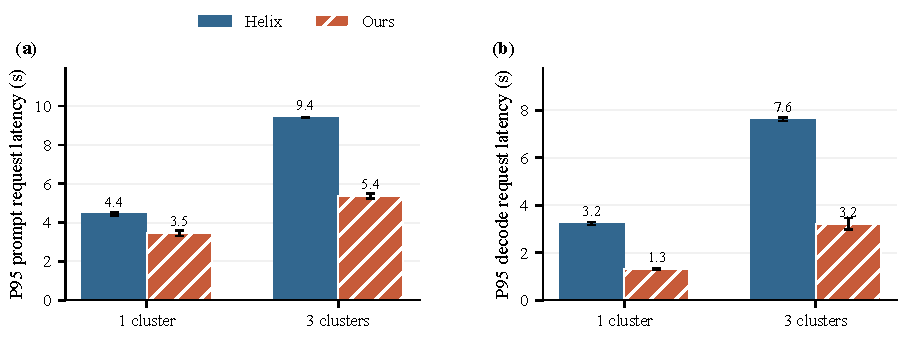
\includegraphics[width=0.95\textwidth]{experiments/paper_figures/fig10_paper_latency.pdf}
\caption{95th-percentile per-request (a) prompt and (b) decode operation latency under the metrics used by the Helix artifact. Conditions match Fig.~\ref{fig:main-performance}; bars show means and sample standard deviations across three paired seeds. These operation-level latencies are distinct from per-query TTFT and TPOT.}
\label{fig:artifact-latency}
\end{figure*}

\begin{figure*}[t]
\centering
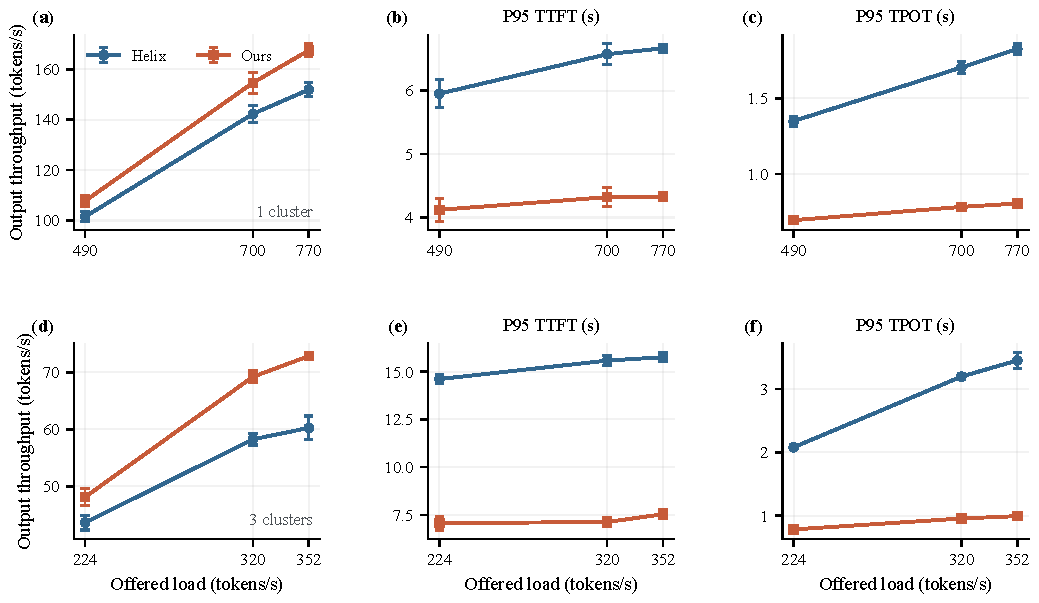
\includegraphics[width=0.95\textwidth]{experiments/paper_figures/fig13_load_sweep.pdf}
\caption{Online serving across offered loads at 0.7, 1, and 1.1 times the Helix artifact setting. Panels (a--c) show single-cluster throughput, P95 TTFT, and P95 TPOT; (d--f) show the same metrics for three clusters. The offered loads are 490/700/770 and 224/320/352 tokens/s, respectively. Each point is the mean of three paired-seed, 1800 s, zero-warmup runs; error bars are sample standard deviations. A separate 1.3-times stress run caused Helix to fail routing within the three-cluster window in all three seeds and is not plotted as a completed throughput point.}
\label{fig:load-sweep}
\end{figure*}

\begin{figure*}[t]
\centering
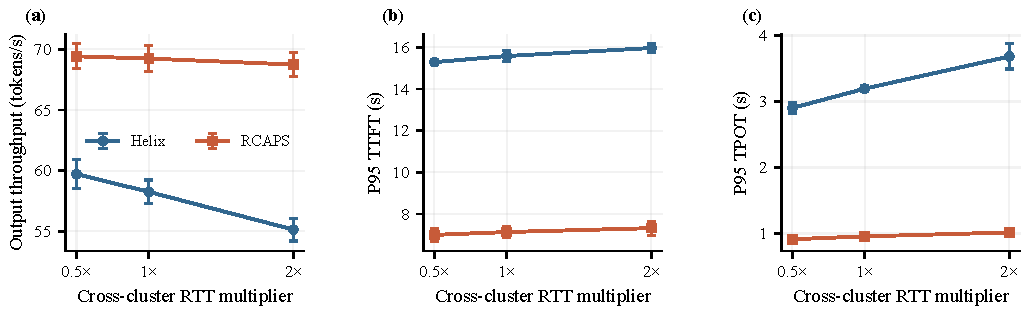
\includegraphics[width=0.95\textwidth]{experiments/paper_figures/fig14_rtt_sensitivity.pdf}
\caption{Three-cluster sensitivity to cross-cluster propagation delay. Only WAN RTT is scaled to 0.5, 1, or 2 times the original configuration; GPU profiles, bandwidth, offered load, and request traces are held fixed. (a) Output-token throughput; (b) P95 TTFT; (c) P95 TPOT. Each point is a three-seed mean with sample-standard-deviation error bars. RCAPS regenerated layer intervals are identical at all three RTTs, so the comparison shows runtime sensitivity under fixed placements.}
\label{fig:rtt-sensitivity}
\end{figure*}

% Supplementary figures.
\begin{figure*}[t]
\centering
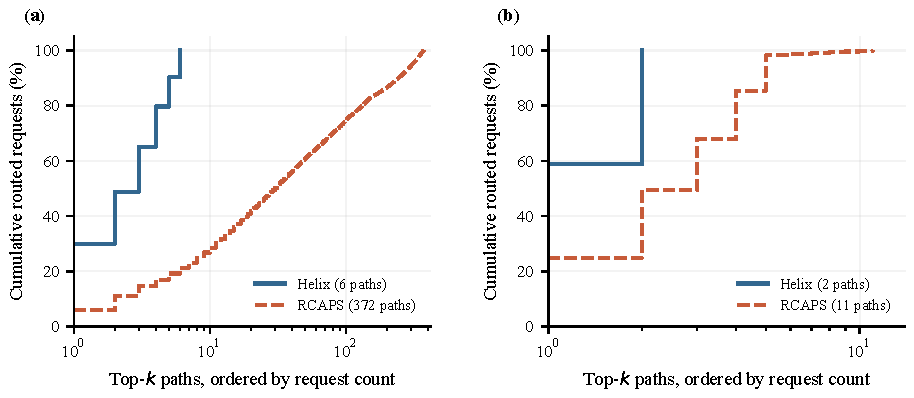
\includegraphics[width=0.95\textwidth]{experiments/paper_figures/fig07_route_concentration.pdf}
\caption{Cumulative share of routed requests carried by the $k$ most frequent GPU paths in (a) one cluster and (b) three clusters. The same official-load seed-0 runs as Fig.~\ref{fig:main-performance} contribute 1291 and 582 first-token queries per arm. The abscissa is logarithmic; path count and diversity are descriptive rather than performance objectives.}
\label{fig:route-concentration}
\end{figure*}

\begin{figure*}[t]
\centering
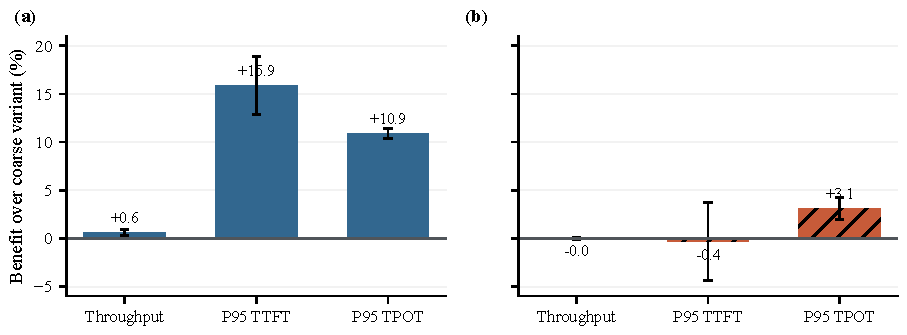
\includegraphics[width=0.95\textwidth]{experiments/paper_figures/fig09_placement_ablation.pdf}
\caption{Internal placement refinement ablation at development loads with the same early layer-DAG scheduler fixed. (a) Single cluster: path-ensemble refinement versus canonical-only placement. (b) Three clusters: critical-path refinement versus the coarse partition. Positive values indicate higher throughput or lower P95 latency; the small negative throughput and TTFT effects in (b) are retained. Bars show paired means and sample standard deviations across seeds 0--2, with 180 s warmup and 1800 s measurement.}
\label{fig:placement-ablation}
\end{figure*}

\begin{figure*}[t]
\centering
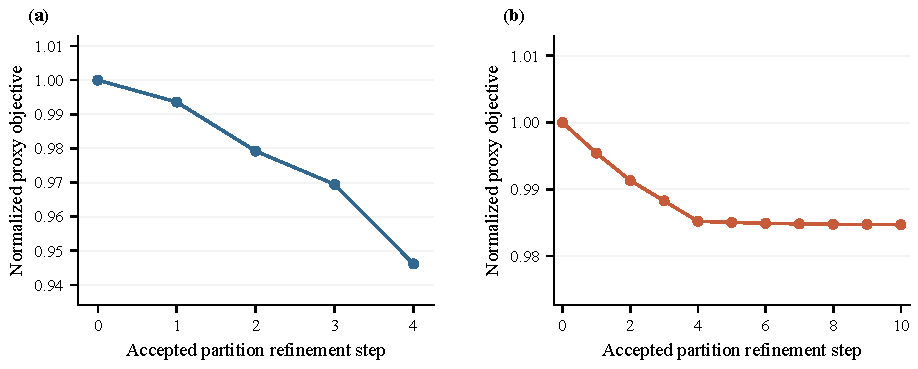
\includegraphics[width=0.95\textwidth]{experiments/paper_figures/fig11_partition_trace.pdf}
\caption{Offline graph-partition search trace for (a) one cluster and (b) three clusters. The ordinate is the normalized analytic objective relative to the coarse partition, which combines estimated TTFT, TPOT, and bottleneck service terms; lower is better. Only accepted moves are plotted. This proxy is not a measured serving latency.}
\label{fig:partition-trace}
\end{figure*}

\begin{figure*}[t]
\centering
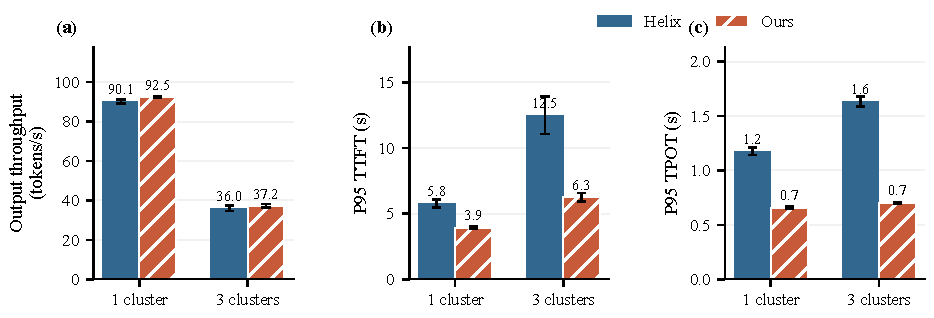
\includegraphics[width=0.95\textwidth]{experiments/paper_figures/fig12_development_load.pdf}
\caption{Separate lower-load end-to-end evaluation, with offered loads of 400 and 160 tokens/s for one and three clusters. (a) Output-token throughput; (b) P95 TTFT; (c) P95 TPOT. Bars show means and sample standard deviations across three paired seeds; each run has 180 s warmup and a fixed 1800 s measurement. This protocol differs from Fig.~\ref{fig:main-performance} and is not joined to it as a load-scaling curve.}
\label{fig:development-load}
\end{figure*}
